\section{Auswertung}
\label{sec:Auswertung}

\subsection{Reflexionsgesetz}

Im ersten Teil des Versuches werden die Reflexionswinkel des grünen Lasers in Abhängigkeit des Einfallswinkels gemessen. Es werden hierzu ein Spiegel und die Messvorlage A
benutzt. Der verwendete Aufbau lässt eine Messung der Winkel auf ein halbes Grad genau zu. Die Ergebnisse der Messung sind in \autoref{tab:refwink} zu finden.

\begin{table}[H]
  \centering
  \caption{Reflexionswinkel.}
  \label{tab:refwink}
  \begin{tabular}{c c c}
    \toprule
    Einfallswinkel / $^{\circ}$ & Ausfallswinkel / $^{\circ}$ & Abweichung / $^{\circ}$\\
    \midrule
    70 & 70$\pm 0,5$ & 0$\pm 0,5$\\
    60 & 55$\pm 0,5$ & 5$\pm 0,5$\\
    50 & 46$\pm 0,5$ & 4$\pm 0,5$\\
    45 & 41$\pm 0,5$ & 4$\pm 0,5$\\
    40 & 37$\pm 0,5$ & 3$\pm 0,5$\\
    30 & 27$\pm 0,5$ & 3$\pm 0,5$\\
    20 & 18$\pm 0,5$ & 2$\pm 0,5$\\
    \bottomrule
  \end{tabular}
\end{table}

\noindent
Es ergibt sich aus den 7 Messwerten eine durchschnittliche Abweichung von $3,0^{\circ}\pm 0,19^{\circ}$. Die Unsicherheit wurde hierbei mit Hilfe von Python berechnet.

\subsection{Brechungsgesetz}

Im zweiten Teil des Versuches soll nun der Brechungsindex von Plexiglas bestimmt werden. Hierfür wird erneut der grüne Laser verwenet. Außerdem eine planparallele
Platte und die Messvorlage A. Um den Brechungsindex zu bestimmen, wird die Gleichung \eqref{eqn:snellius} genutzt, wobei $n_1 = 1$ angenommen wird und $n_2$ der
zu bestimmende Index ist. Die Ergebnisse der 7 Messungen sind zusammen mit dem daraus resultierenden Index in \autoref{tab:brech} dargestellt.

\begin{table}[H]
  \centering
  \caption{Brechungsindex.}
  \label{tab:brech}
  \begin{tabular}{c c c}
    \toprule
    Einfallswinkel / $^{\circ}$ & Ausfallswinkel / $^{\circ}$ & Brechungsindex \\
    \midrule
    70 & 38$\pm 0,5$ & 1,53$\pm 0,022$\\
    60 & 36$\pm 0,5$ & 1,47$\pm 0,022$\\
    50 & 31$\pm 0,5$ & 1,49$\pm 0,025$\\
    45 & 28,5$\pm 0,5$ & 1,48$\pm 0,027$\\
    40 & 26$\pm 0,5$ & 1,47$\pm 0,029$\\
    30 & 19,5$\pm 0,5$ & 1,50$\pm 0,040$\\
    20 & 13,5$\pm 0,5$ & 1,47$\pm 0,050$\\
    10 & 7$\pm 0,5$ & 1,42$\pm 0,100$\\
    \bottomrule
  \end{tabular}
\end{table}

\noindent
Als Mittelwert folgt daraus für den Brechungsindex $n = 1,48 \pm 0,017$. Mit Gleichung \eqref{eqn:geschw} folgt daraus für die Lichtgeschwindigkeit in Plexiglas
$v = (2,026 \pm 0,023) \cdot 10^8 \si{\meter\per\second}$. Die Unsicherheiten wurden erneut mit Hilfe von Python berechnet.

\subsection{Prisma}

Im nächsten Teil des Versuches soll die Ablenkung eines Prismas untersucht werden. Dazu wird ein Prisma aus Kronglas, ein grüner und roter Laser und die Messvorlage C
verwendet. Die Ablenkung wird mit Hilfe von Gleichung \eqref{eqn:prismaWinkel}, mit der Winkelbeziehung $\beta_1 + \beta_2 = \gamma$ bestimmt. $\gamma$ wird
als brechender Winkel bezeichnet und ist bei dem verwendeten Prisma gegeben als $\gamma = 60^{\circ}$.
\newline
Die gemessenen Werte sind in \autoref{tab:prisma} zu finden.

\begin{table}[H]
  \centering
  \caption{Prisma.}
  \label{tab:prisma}
  \begin{tabular}{c c c}
    \toprule
    Einfallswinkel / $^{\circ}$ & Austrittswinkel Rot / $^{\circ}$ & Austrittswinkel Grün / $^{\circ}$\\
    \midrule
    55 & 42$\pm 0,5$ & 43$\pm 0,5$\\
    50 & 47$\pm 0,5$ & 48$\pm 0,5$\\
    45 & 53$\pm 0,5$ & 53$\pm 0,5$\\
    40 & 59$\pm 0,5$ & 60$\pm 0,5$\\
    35 & 67$\pm 0,5$ & 68$\pm 0,5$\\
    \bottomrule
  \end{tabular}
\end{table}

\noindent
Die daraus folgenden Ablenkungen sind für den roten und grünen Laser in \autoref{tab:abl} dargestellt. Die Unsicherheiten wurden erneut mit Python bestimmt.

\begin{table}[H]
  \centering
  \caption{Prisma.}
  \label{tab:abl}
  \begin{tabular}{c c }
    \toprule
    Ablenkung Rot / $^{\circ}$ & Ablenkung Grün / $^{\circ}$\\
    \midrule
    37$\pm 0,5$ & 38$\pm 0,5$\\
    37$\pm 0,5$ & 38$\pm 0,5$\\
    38$\pm 0,5$ & 38$\pm 0,5$\\
    39$\pm 0,5$ & 40$\pm 0,5$\\
    42$\pm 0,5$ & 43$\pm 0,5$\\
    \bottomrule
  \end{tabular}
\end{table}

\noindent
Daraus folgen die Mittelwerte $\delta_\text{Rot} = 38,6^{\circ} \pm 0,22^{\circ}$ und $\delta_\text{Grün} = 39,4^{\circ} \pm 0,22^{\circ}$.

\subsection{Beugung am Gitter}

Im letzten Teil des Versuches soll die Wellenlänge der verwendeten Laser durch die Beugung an verschiedenen Gittern ermittelt werden. Dafür werden drei verschiedenen
Gitter mit 600, 300 und 100 Linien pro Millimeter und die beiden Laser verwendet. Die Messwerte für 100 Linien pro Millimeter sind in \autoref{tab:git100}, die
für 300 in \autoref{tab:git300} und die für 600 in \autoref{tab:git600} zu finden.
\newline
Die Wellenlängen lassen sich nun anhand von Gleichung \eqref{eqn:lambda} bestimmen.

\begin{table}[H]
  \centering
  \caption{Gitter 100.}
  \label{tab:git100}
  \begin{tabular}{c c c}
    \toprule
    Ordnung & Beugungswinkel Rot / $^{\circ}$ & Beugungswinkel grün / $^{\circ}$\\
    \midrule
    1 & 3$\pm 0,5$ & 2,5$\pm 0,5$\\
    2 & 5,5$\pm 0,5$ & 4,5$\pm 0,5$\\
    3 & 8$\pm 0,5$ & 6,5$\pm 0,5$\\
    4 & 11$\pm 0,5$ & 9$\pm 0,5$\\
    5 & 14$\pm 0,5$ & 11,5$\pm 0,5$\\
    6 & 17$\pm 0,5$ & 14$\pm 0,5$\\
    7 & 20$\pm 0,5$ & 16$\pm 0,5$\\
    \bottomrule
  \end{tabular}
\end{table}

\noindent
Für das Gitter mit 100 Linien pro Millimeter ergibt sich $\lambda_\text{Rot} = (4,86 \pm 0,15) \cdot 10^9 \si{\meter}$ und
$\lambda_\text{Grün} = (3,99 \pm 0,15) \cdot 10^9 \si{\meter}$.

\begin{table}[H]
  \centering
  \caption{Gitter 300.}
  \label{tab:git300}
  \begin{tabular}{c c c}
    \toprule
    Ordnung & Beugungswinkel Rot / $^{\circ}$ & Beugungswinkel grün / $^{\circ}$\\
    \midrule
    1 & 8 & 6,5\\
    2 & 16,5 & 13,5\\
    3 & 25,5 & 21\\
    \bottomrule
  \end{tabular}
\end{table}

\noindent
Für das Gitter mit 300 Linien pro Millimeter ergibt sich $\lambda_\text{Rot} = (1,416 \pm 0,034) \cdot 10^8 \si{\meter}$ und
$\lambda_\text{Grün} = (1,165 \pm 0,15) \cdot 10^8 \si{\meter}$.

\begin{table}[H]
  \centering
  \caption{Gitter 600.}
  \label{tab:git600}
  \begin{tabular}{c c c}
    \toprule
    Ordnung & Beugungswinkel Rot / $^{\circ}$ & Beugungswinkel grün / $^{\circ}$\\
    \midrule
    1 & 16,5 & 13,5\\
    2 & & 29,5\\
    \bottomrule
  \end{tabular}
\end{table}

\noindent
Für das Gitter mit 600 Linien pro Millimeter ergibt sich $\lambda_\text{Rot} = (2,40 \pm 0,05) \cdot 10^8 \si{\meter}$ und
$\lambda_\text{Grün} = (2,84 \pm 0,09) \cdot 10^8 \si{\meter}$.
\newline \newline
Aus allen drei Messreihen ergibt sich so als Mittelwert $\lambda_\text{Rot} = (1,434 \pm 0,021) \cdot 10^8 \si{\meter}$ für den roten und
$\lambda_\text{Grün} = (1,47 \pm 0,06) \cdot 10^8 \si{\meter}$ für den grünen Laser.

\printbibliography{}

\section*{Anhang}
\label{sec:anhang}

\begin{figure}[H]
  \centering
  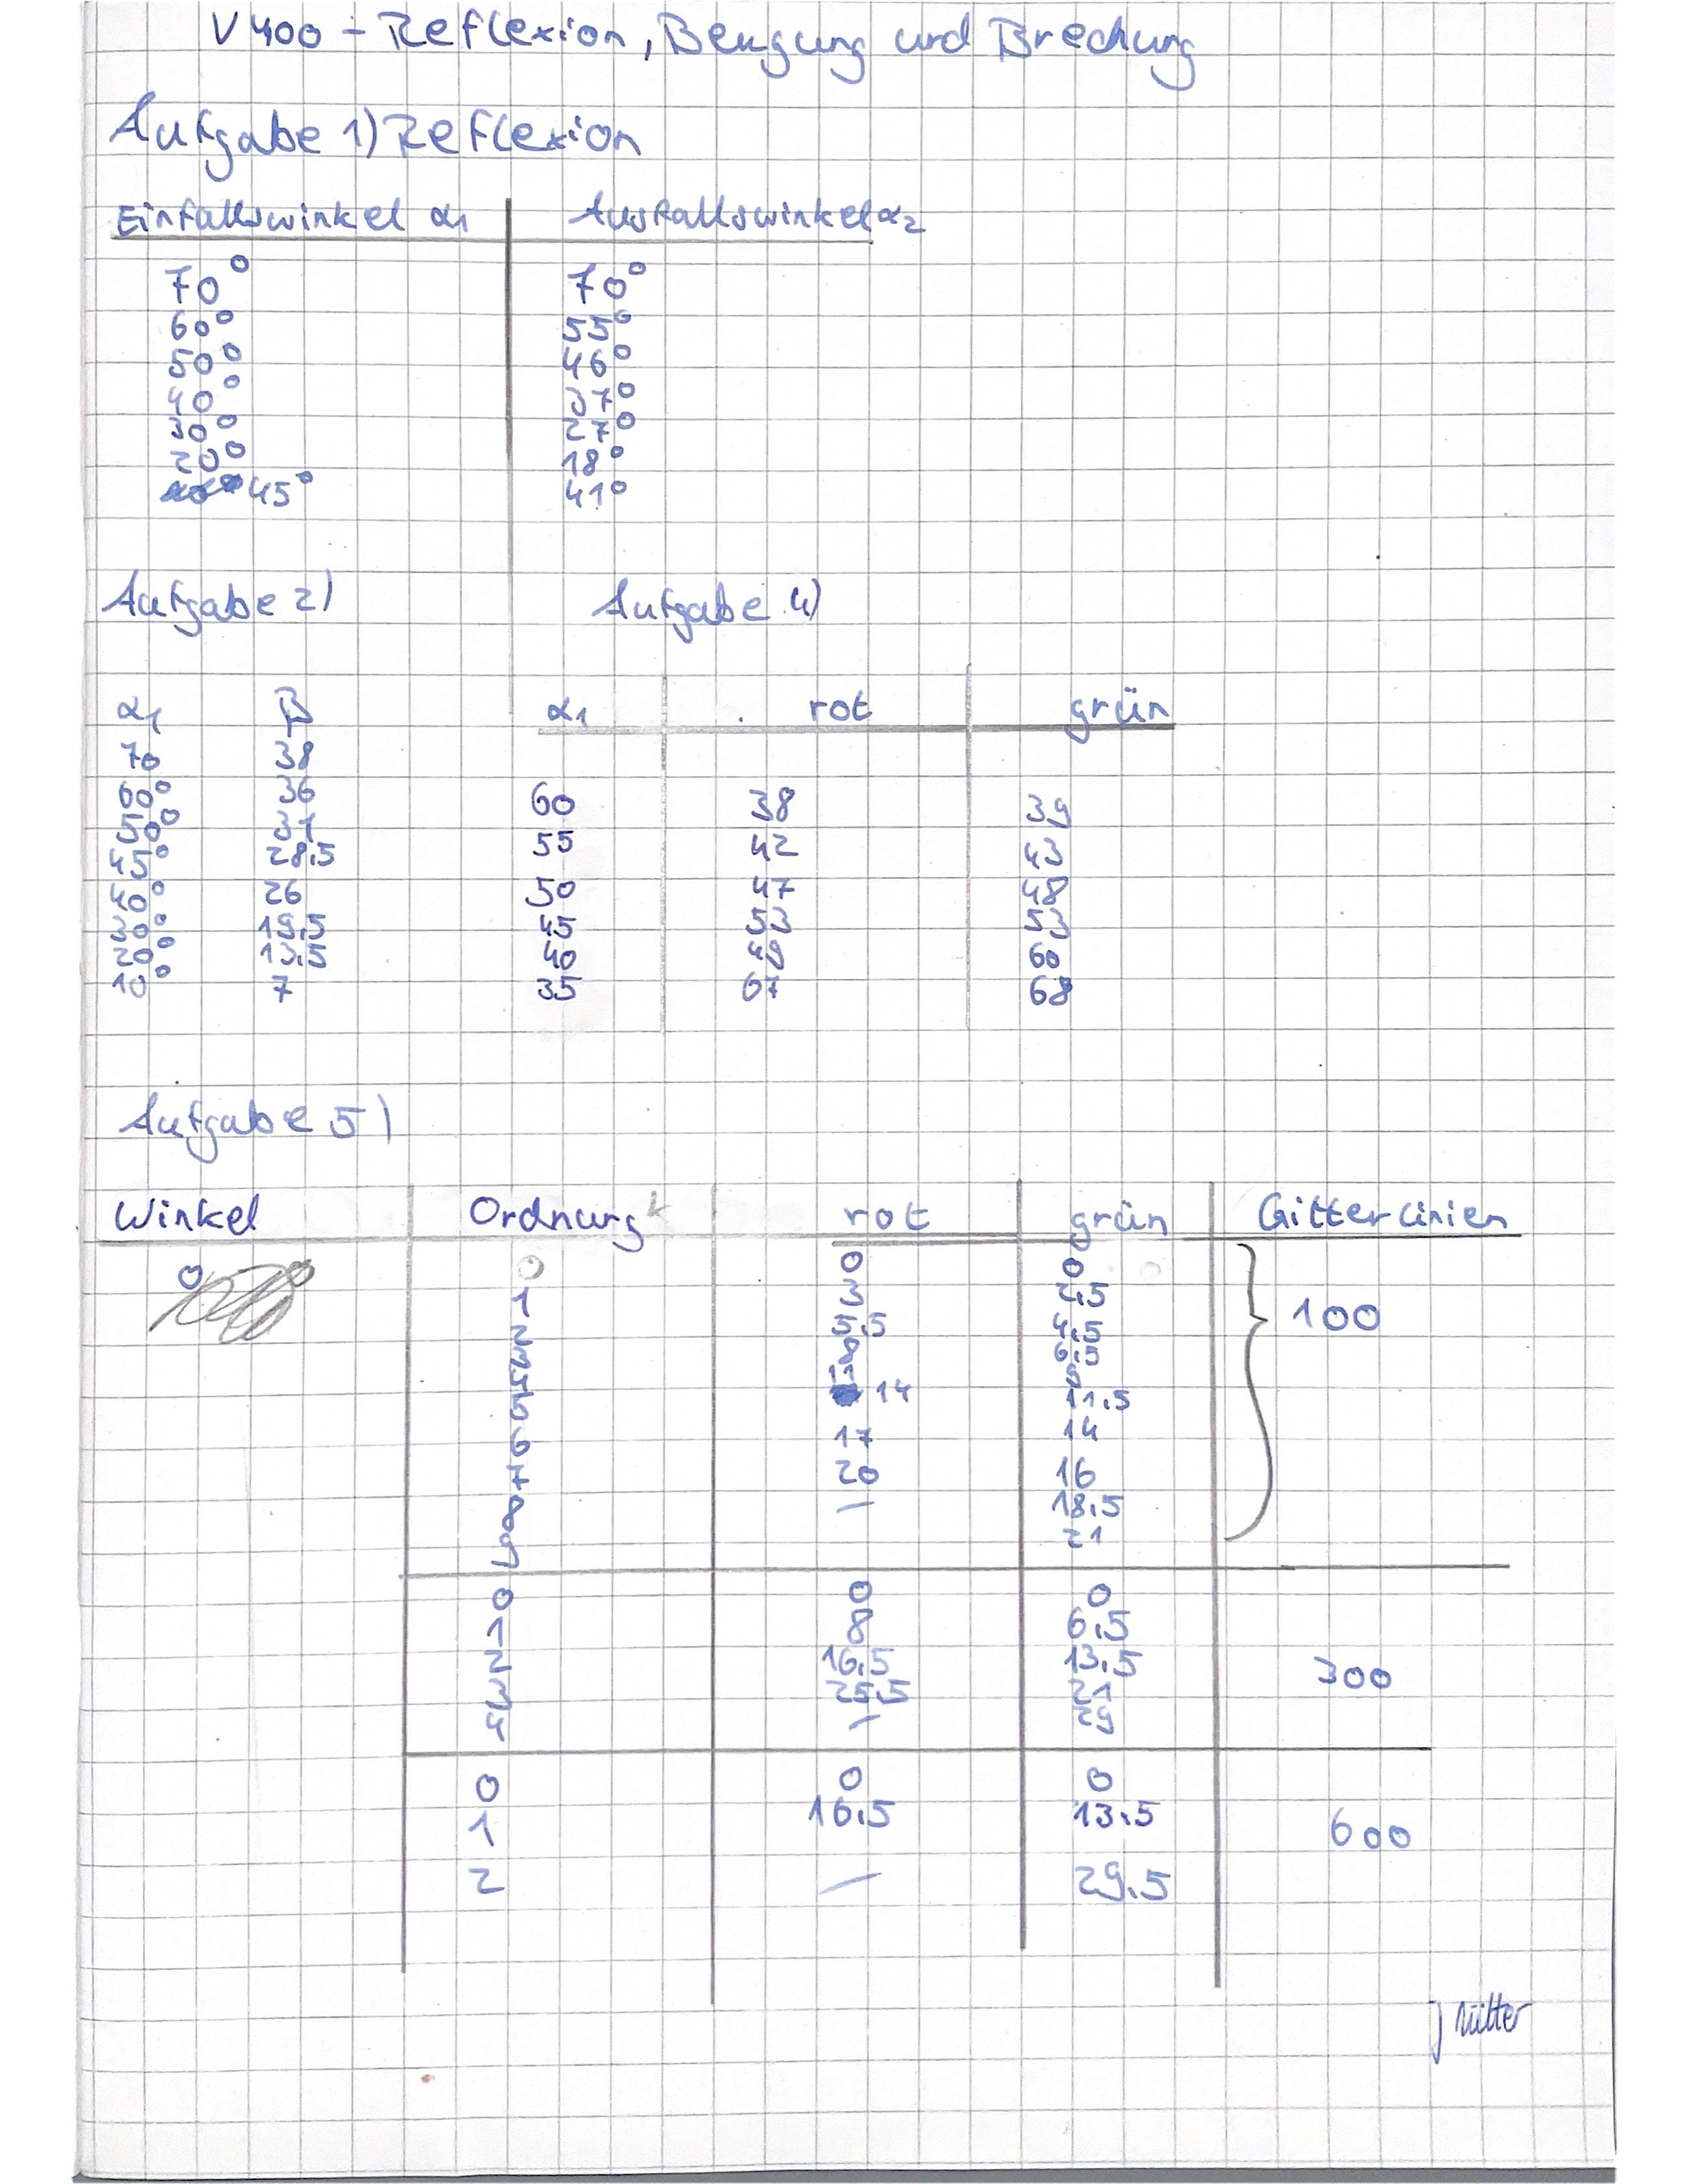
\includegraphics[width=0.7\textwidth]{data/origDaten.jpg}
  \caption{Originale Messdaten.}
  \label{fig:origDaten1}
\end{figure}